% !TeX root = ../../main.tex
% Add the above to each chapter to make compiling the PDF easier in some editors.

\section{Generalization over users}\label{ord:ch5:sec_3_generalization_user}

% RE-1468


% Variance for IoU of the single methods to compare which method is the most reliable around various users
% Variance for Time of the single methods
\subsection{Benchmark Participants Evaluation}\label{ord:ch5:sec3:subsec1}

% Motivation: generalization over user -> an interactive method really performs well and reliable if it delivers good results for all possible users.

% Compare the variance of the methods based on all users and all real benchmark users

% Compare the variance of single users per method
% Test how stable the variance is

\subsection{Two Experienced User} \label{ord:ch5:sec3:subsec2_cmo_afe}

% No significant difference in the IoU between the two user could be detected -> generalize well over various users (few user, large data)

\begin{table}[h!]
	\centering
	\resizebox{\textwidth}{!}{
		\begin{tabular}{l|c c}
			\toprule 		
							& Kruskal-Wallis test 	& Mann-Whitney U-test \\
			\midrule
			$ H_{0} $			& $ med \left( IoU_{\textnormal{\textit{User 1}}} \right)  = med \left( IoU_{\textnormal{\textit{User 2}}} \right) $ & $ t_{{\textnormal{\textit{User 1}}}} = t_{\textnormal{\textit{User 1}}} $ 		\\
			$ H_{A} $		& $ med \left( IoU_{classical} \right) \not= med \left( IoU_{dl} \right) $ &  $ t_{{\textnormal{\textit{User 1}}}} \not= t_{\textnormal{\textit{User 1}}} $ 	\\
			$ \alpha $		& $ 5\% $ 		 		& $ 5\% $ 		\\ 	
			Statistics		& 1.9246	     		& 5294.5    	\\ 
			$ \textnormal{\textit{p-value}} $ 
							& 0.1654	 		 	& 0.0828		\\ 
			$ H_{0} $		& accepted		 		& accepted 		\\
			\bottomrule
	\end{tabular}}
	\caption[Hypothesis Tests on $ IoU $ for the Watersheds method]{
		For the method $ Watersheds $ this is an exemplary overview of the two statistical tests performed on the variable $ IoU $.
		The variable $ IoU $ is evaluated by the median and tendency of the sample.
		Each factor contains 109 annotations.
		If the $ \textnormal{\textit{p-value}} $ is greater than the significance level $ \alpha = 5\% $, $ H_{0} $ is accepted.
		Both, the Kruskal-Wallis test and the Mann-Whitney U-test accept the null hypothesis, that there are no statistical significant differences between the methods.
		For the \gls{dextr} and \gls{iog} method equivalent tests were performed on the same setup, which all accepted $ H_{0} $.
	}\label{tab:ch5:tests_afe_cmo}	
\end{table}
% TODO include polygon run
% TODO Include number of annotations?

\begin{figure}
	\centering
	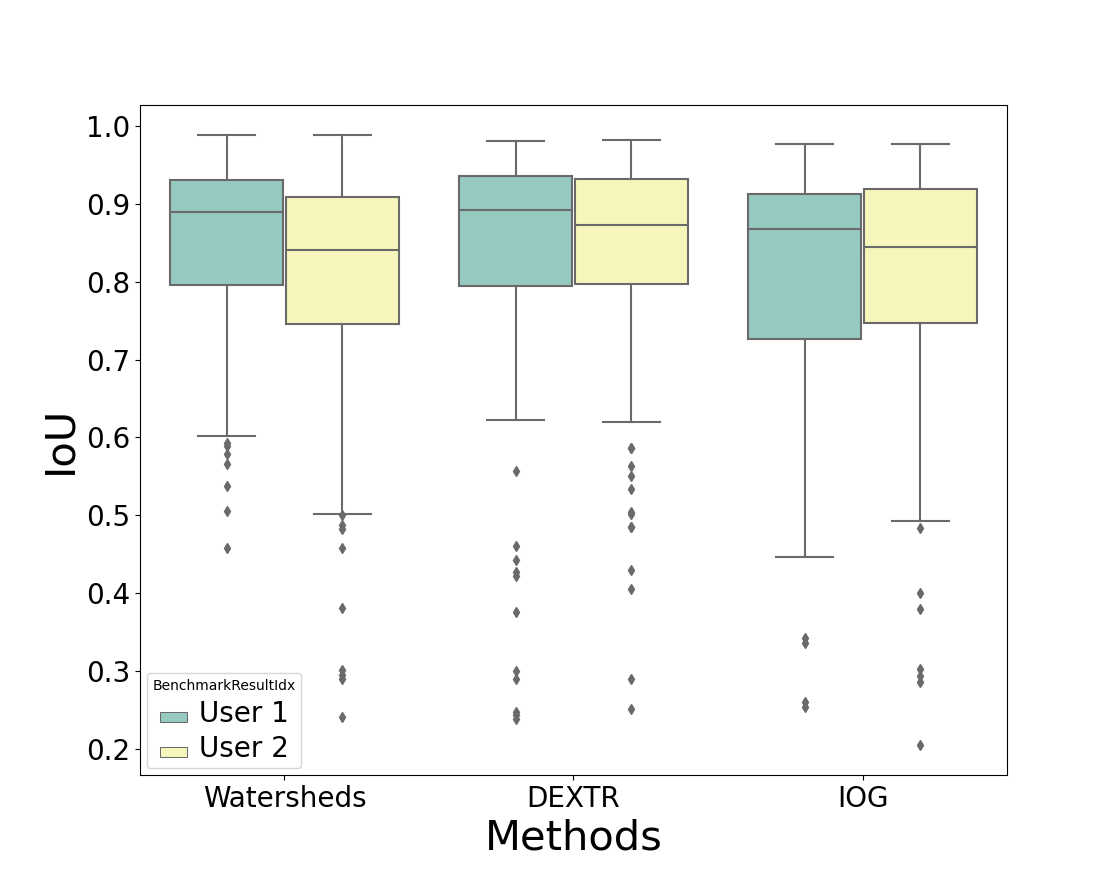
\includegraphics[width=0.9\textwidth]{figures/chap53_afe_cmo.png}
	\caption[tbd]{
		tbd.
	} \label{fig:ch5:sec3:cmo_afe}
\end{figure}
% TODO add Polygon (and keep the methods soerted)


\subsection{Simulations With Different Click Patterns / Noise}\label{ord:ch5:sec3:subsec3}
% RE-1468

% Simulations are easily scalable, faster and cheaper than the acquisition of manual clicks from real users.
% Second, in a simulation no variance occurs between the set clicks of various users, if the .
% Third, simulations have the possibility to effortless create various click patterns, that \eg vary the set click by a random offset, in order to simulate a various types of user behavior.
%On the other hand, simulations are only capable to replicate the user's behavior to a certain extent.
% Further, the involvement of human users is especially important for methods, which performance depends on user interactions.


In order to gain deeper insights on the functionality of the \gls{dextr} and \gls{iog} method the simulation setup is modified.
% Motivation - Nachahmung von unterschiedlichen Usertypen durch unterschiedliche Genauigkeit bei der Klick-Simulation.
The altered simulation setup uses different levels of accuracy, to simulate more realistic user clicks.
% Simulation of with different permutation / deviation / - simulation of different user

The level of accuracy is defined by a deviation of maximal $ n_{deviation} $ \Unit{px}.
In the range $ \left[-n_{deviation}, \dots, 0, \dots, n_{deviation} \right] $ two values are randomly selected and added to the ideal row and column.
This random factor was added, to simulate the varying accuracy of single user clicks.
The smaller $ n_{deviation} $, the more accurate are the simulated clicks.
In the simulation first the ideal click position is calculated and further the random deviation is added.
This procedure is applied to the extreme points of the \gls{dextr} method and to the fore- and background clicks of the \gls{iog} method.
\begin{table}[h!]
	\centering	
	\resizebox{\textwidth}{!}{
	\begin{tabular}{l l|c c c c c c c}
		\toprule
				&							& \multicolumn{7}{c}{mIoU} \\
				& {$ n_{deviation} $} 		& 0	\Unit{px}	& 5	\Unit{px}	& 10 \Unit{px}	& 15 \Unit{px}	& 20 \Unit{px}	& 25 \Unit{px}	& 30 \Unit{px}	\\
		\midrule
		DEXTR 	& PASCAL (VP \cmark)	& 0.9103	& 0.8323	& 0.7626	& 0.7032 	& 0.6479	& 0.6047	& 0.5626		\\
				& PASCAL (VP \xmark)	& 0.7807	& 0.7523	& 0.7019	& 0.6543 	& 0.6085	& 0.5695	& 0.5317		\\
				& Benchmark			& 0.8414	& 0.7743	& 0.6887	& 0.6240 	& 0.5579	& 0.5027	& 0.4892		\\
		\midrule
		IOG 	& PASCAL (VP \cmark)	& 0.9267	& 0.8846	& 0.8092	& 0.7352 	& 0.6578	& 0.5953 	& 0.5457		\\
				& PASCAL (VP \xmark)	& 0.8081	& 0.7720	& 0.7099	& 0.6476 	& 0.5979	& 0.5337	& 0.4873		\\
				& Benchmark			& 0.8219	& 0.7865	& 0.7173	& 0.6027 	& 0.5268	& 0.4493 	& 0.4058		\\
		\bottomrule
	\end{tabular}}
	\caption[Simulations with different click patterns]{
		Simulations of the \gls{dextr} and \gls{iog} method with user clicks, that are simulated with varying degrees of accuracy.
		The parameter $ n_{deviation} $ states the maximal possible deviation from the optimal point, in order to mimic different types of users.
		As expected, the performance decreases with increasing deviation in the simulated user clicks.
	}\label{tab:ch5:simulation_various_click_patterns}
\end{table}
%TODO benchmark performance of real users for IOG and DEXTR is at 89% and 87% mIoU, while the best simulation is only at 84% and 82% mIoU - das passt nicht so wirklich zusammen.

The performance constantly decreases with higher $ n_{deviation} $, as demonstrated in Table \ref{tab:ch5:simulation_various_click_patterns}. 
Even a comparable small deviation of maximal 5 \Unit{px} leads a notable drop in performance.
This factor needs to be taken into account, if these methods are applied by real users.




